\documentclass[polish,polish,a4paper]{article}
\usepackage{cmap}

\usepackage[T1]{fontenc}
\usepackage[utf8]{inputenc}
\usepackage{listings}
\usepackage{graphicx} 
\usepackage{tikz}
\usepackage{xcolor}
\usepackage{babel}
\usepackage{pslatex}
\usepackage{tikz}
\usepackage{pgfplots}
\usepackage{anysize}
\usepackage{pgfgantt}
\usepackage{latexsym,amsmath}

\marginsize{2.5cm}{2.5cm}{3cm}{3cm}
\graphicspath{ {D:\Nauka\Grafika Komputerowa\lab4 światło\latex} }


\title{Sprawozdanie nr 5, Teksturowanie}
\author{Łukasz Szumilas, Grupa E02-81o}
\date{Zajęcia: 19.12.2018 (odrobione 28 stycznia)}

\begin{document}
  \begin{center}\Large
    Grafika Komputerowa i Komunikacja Człowiek-Komputer
  \end{center}
  \hrule
  {\let\newpage\relax\maketitle}
  \hrule


  \section{Omówienie tematu}
  Celem ćwiczenia było pokazanie podstawowych technik teksturowania powierzchni obiektów z wykorzystaniem mechanizmów biblioteki OpenGL z rozszerzeniem GLUT. Zostało przedstawione krok po kroku odpowiednie wczytywanie teksturyz obrazka o odpowiednim formacie. Teksturowanie odbyło się na przykładach trójkąta, wielościanu i  bardziej skomplikowanego modelu w postaci siatki trójkątów (jajka).
\\\indent Na rozgrzewkę, przy użyciu programów z poprzednich laboratoriów, należało przedstawić biały trójkąt oświetlony białym światłem. Wykorzystany był program napisany w ćwiczeniu 4  pozwalający obserwować figurę z punktu na powierzchni sfery. Dla ilustracji 
oświetlenia pomocne były instrukcje z ćwiczenia 5.  Efekty widać na \textbf{\textit{rysunku nr 1}}.
\\\indent Po wykonaniu tej części należało wstawić teksturę na oświetlony trójkąt przy użyciu gotowej funkcji \textit{GLbyte *LoadTGAImage}, należało także dopisać kilka linii kodu w funkcji \textit{MyInit()}, zawierającego podstawowe funkcje definiujące właściwości teksturowania. Ważne było wprowadzenie odpowiednich współrzędnych wzorca tekstury definiującej fragment obrazu, jaki ma być naniesiony na powierzchnię trójkąta. Efekt tego przedsięwzięcia widnieje na \textbf{\textit{rysunku nr 2}}. Dzięki informacjom wyniesionym z laboratorium `Interakcja z użytkownikiem' trójkąt można obracać, dzięki temu lepiej można zbadać wczytaną teksturę (\textbf{\textit{rysunek nr 3}}). 
\\\indent Następnym etapem było obłożenie teksturą figury 3D,ostrosłupa. W funkcji \textit{RenderScene()}, dzięki odpowiednim połączeniu zdefiniowanych punktów w przestrzeni trójwymiarowej  można było połączyć cztery pochylone trójkąty z podstawą kwadratu, łącząc w ten sposób ostrosłup. Z racji tego, że teksturowanie było prowadzone tylko po jednej stronie każdej ściany, trzeba było mieć na uwadzę odpowiednią kolejność łączonych punktów. Najważniejsze rzeczy zostały zawarte \textbf{\textit{kodzie nr 1 i rysunku nr 4}}.
\\\indent Nakładanie tekstury na figurę jajka było o tyle trudniejsze, że figura ta nie ma płaskiej powierzchni i bez odpowiedniego rozplanowania punktów tekstury w \textit{glTexCoord2f(..)} obraz może być całkowicie nieczytelny. Tekstura została pokryta taką samą siatką trójkątów jaką naniesiono na dziedzinę parametryczną, z zachowaniem odpowiedniej kolejności. Tekstury w formacie \textit{tga} były przygotowane specjalnie do tego laboratorium, ale nic nie stoi na przeszkodzie w zdefiniowaniu własnej, przy konwersji pliku w odpowiednio dedykowanym do tego programie. W tym przypadku pomocna była strona \textit{https://www.online-convert.com}. Efekt: \textbf{\textit{rysunek nr 5 i 6}}. 
  \section{Omówienie kodu}
   \textbf{Kod 1}, fragment funkcji \textit{RenderScene()}.
{\small
\begin{lstlisting}[language=C++]
	glColor3f(1.0f, 1.0f, 1.0f);//kolor bialy
	

	glBegin(GL_QUADS);

	glTexCoord2f(1.0f, 0.0f);
	glVertex3f(5.0f, 0.0f, 5.0f);

	glTexCoord2f(0.0f, 0.0f);
	glVertex3f(-5.0f, 0.0f, 5.0f);

	glTexCoord2f(0.0f, 1.0f);
	glVertex3f(-5.0f, 0.0f, -5.0f);

	glTexCoord2f(1.0f, 1.0f);
	glVertex3f(5.0f, 0.0f, -5.0f);
	
	glEnd();


	glBegin(GL_TRIANGLES);

	glTexCoord2f(0.5f, 2.0f);
	glVertex3f(0.0f, 10.0f, 0.0f);

	glTexCoord2f(0.0f, 0.0f);
	glVertex3f(5.0f, 0.0f, 5.0f);

	glTexCoord2f(1.0f, 0.0f);
	glVertex3f(5.0f, 0.0f, -5.0f);


	glBegin(GL_TRIANGLES);

	glTexCoord2f(1.0f, 0.0f);
	glVertex3f(-5.0f, 0.0f, 5.0f);

	glTexCoord2f(0.5f, 2.0f);
	glVertex3f(0.0f, 10.0f, 0.0f);

	glTexCoord2f(0.0f, 0.0f);
	glVertex3f(-5.0f, 0.0f, -5.0f);

	glEnd();

	glBegin(GL_TRIANGLES);

	glTexCoord2f(1.0f, 0.0f);
	glVertex3f(-5.0f, 0.0f, 5.0f);

	glTexCoord2f(0.0f, 0.0f);
	glVertex3f(5.0f, 0.0f, 5.0f);

	glTexCoord2f(0.5f, 2.0f);
	glVertex3f(0.0f, 10.0f, 0.0f);

	glEnd();

	glBegin(GL_TRIANGLES);

	glTexCoord2f(1.0f, 0.0f);
	glVertex3f(-5.0f, 0.0f, -5.0f);

	glTexCoord2f(0.5f, 2.0f);
	glVertex3f(0.0f, 10.0f, 0.0f);

	glTexCoord2f(0.0f, 0.0f);
	glVertex3f(5.0f, 0.0f, -5.0f);

	glEnd();

	glFlush();
	glutSwapBuffers();

\end{lstlisting}
}
\textbf{Kod 2}, nakladanie tekstury na jajko.
{\small
\begin{lstlisting}[language=C++]
//i, j - kolejne punkty w przestrzeni dwuwymiarowej (0:1) 
//dla ktorych obliczane byly wartosci dla jajka
//N - liczba podzialu tej przestrzeni, w tym przypadku N = 100

//pominiete fragmenty dot. oswietlenia, obrotu i 
//obliczania wspolrzednych jajka, wykorzystane z poprzednich lab
//i zawarte w poprzednich sprawozdaniach
	if (i > 0 && j > 0) {
				glBegin(GL_TRIANGLES);
				glTexCoord2f(i / N, j / N);
				glVertex3fv(tabXYZ[i][j]);

				glTexCoord2f((i + 1) / N, j / N);
				glVertex3fv(tabXYZ[(i + 1)][j]);


				glTexCoord2f(i / N, (j + 1) / N);
				glVertex3fv(tabXYZ[i][j + 1]);

				glEnd();

				glBegin(GL_TRIANGLES);
				glTexCoord2f((i + 1) / N, j / N);
				glVertex3fv(tabXYZ[(i + 1)][j]);

				glTexCoord2f((i + 1) / N, (j + 1) / N);
				glVertex3fv(tabXYZ[(i + 1)][j + 1]);

				glTexCoord2f(i / N, (j + 1) / N);
				glVertex3fv(tabXYZ[i][j + 1]);

				glEnd();
			}
}
\end{lstlisting}
}


  \section{Rezultat prac}

    \begin{figure}[h!]
      \centering
      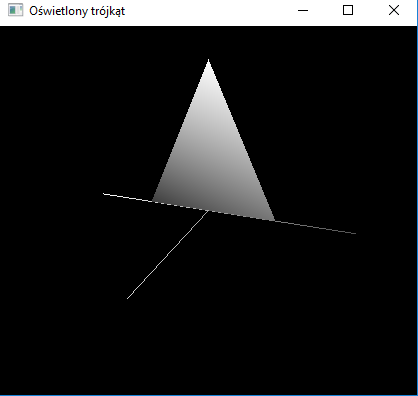
\includegraphics[width=0.6\textwidth,height=8cm]{oswietlonytrojkat.png}
      \caption{Oświetlony trójkąt. Białe światło, biały kolor.}
      \label{fig:zrzut1}
    \end{figure}

    \begin{figure}[h!]
      \centering
      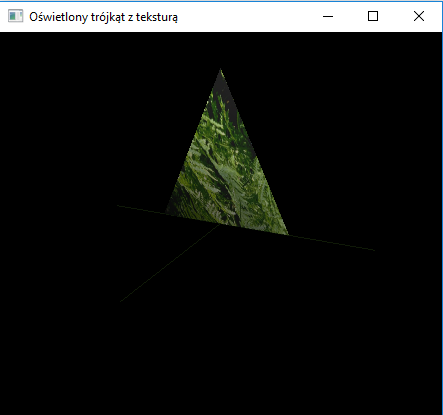
\includegraphics[width=0.6\textwidth,height=8cm]{oswietlonytrojkattekstura.png}
      \caption{Nałożona tekstura na trójkąt.}
      \label{fig:zrzut1}
    \end{figure}

    \begin{figure}[h!]
      \centering
      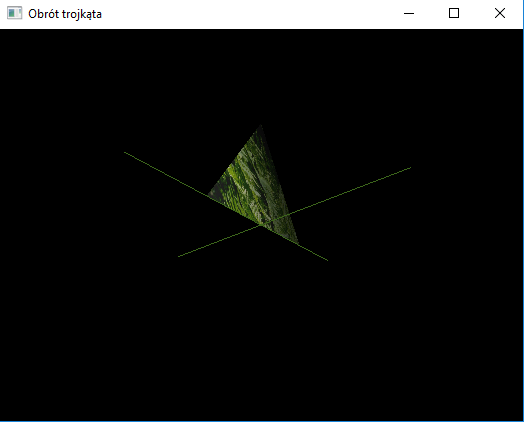
\includegraphics[width=0.6\textwidth,height=8cm]{obrottrojkata.png}
      \caption{Obrócony trójkąt.}
      \label{fig:zrzut1}
    \end{figure}

    \begin{figure}[h!]
      \centering
      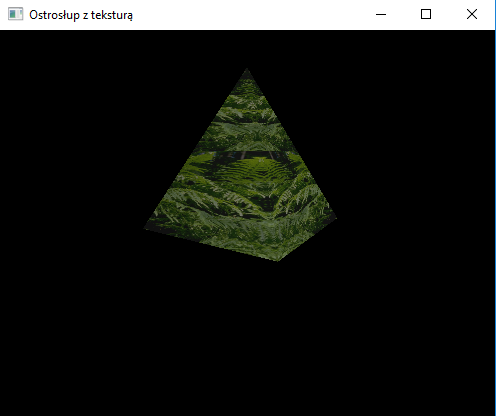
\includegraphics[width=0.6\textwidth,height=8cm]{ostroslupztekstura.png}
      \caption{Ostrosłup z nałożoną teksturą.}
      \label{fig:zrzut1}
    \end{figure}
    
        \begin{figure}[h!]
      \centering
      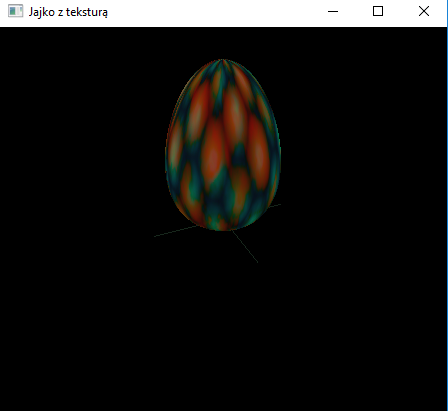
\includegraphics[width=0.6\textwidth,height=8cm]{jajkoztekstura.png}
      \caption{Jajko z teksturą.}
      \label{fig:zrzut1}
    \end{figure}
    
            \begin{figure}[h!]
      \centering
      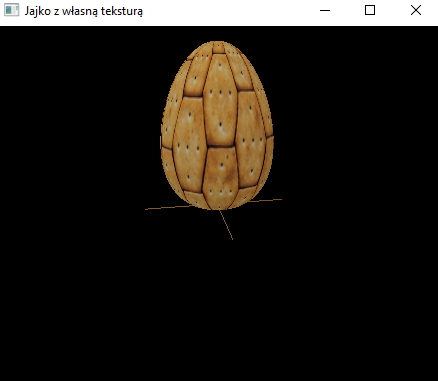
\includegraphics[width=0.6\textwidth,height=8cm]{jajkozwlasnatekstura.png}
      \caption{Jajko z własną teksturą.}
      \label{fig:zrzut1}
    \end{figure}


\end{document}